\setcounter{rownumber}{0}
\singlespacing
\chapter{Brillouin-Induced Raman Modes and Device Exploration}
\label{ch:Raman}
\acresetall

\doublespacing

%%%%%%%%%%%%%%%%%%%%%%%%%%%%%%%%%%%%%%%%%%%%%%%%%%%%%%%%%%%%%%%%%%%%

\section{Introduction}
\label{sec:Raman:Introduction}

\begin{itemize}
  \item \textbf{Motivation and Context}
  \begin{itemize}
    \item Summarize the overarching goal: demonstrating Brillouin-induced Raman modes at room temperature and exploring the transition from traveling-wave (Brillouin) to standing-wave (Raman-like) phonons.
    \item Place this research in the broader context of optomechanics and light--matter interactions, referencing how earlier chapters (especially the laser cooling chapter) set the stage for advanced phonon manipulation.
    \item Note that, unlike your two ``wins'' in prior chapters, this work did not yield a final demonstration but yielded significant progress toward that goal.
  \end{itemize}
\end{itemize}

%--------------------------------------------------------------------%

\section{From Traveling-Wave to Raman-Like Standing-Wave Modes}
\label{sec:Raman:FromTraveling-WavetoRaman-LikeStanding-WaveModes}

\subsection{Review of Brillouin and Raman Scattering}
\label{subsec:Raman:ReviewofBrillouinandRamanScattering}

\begin{itemize}
  \item Recap key concepts: Brillouin scattering (traveling acoustic waves) and Raman scattering (molecular/lattice vibrational modes).
  \item Emphasize how confined geometries can turn traveling phonons into standing waves, potentially shifting the Brillouin regime to a Raman-like regime.
\end{itemize}

\subsection{Brillouin-Induced Raman Modes}
\label{subsec:Raman:Brillouin-InducedRamanModes}

\begin{itemize}
  \item Present the theoretical argument that traveling-wave phonons (driven by stimulated Brillouin scattering) can reflect off boundaries to form standing waves, creating Raman-like discrete modes.
  \item Outline expected spectral signatures: mode spacing tied to path length and sound speed, resembling a harmonic ladder of vibrational modes.
\end{itemize}

\begin{figure}[t]
  \centering
  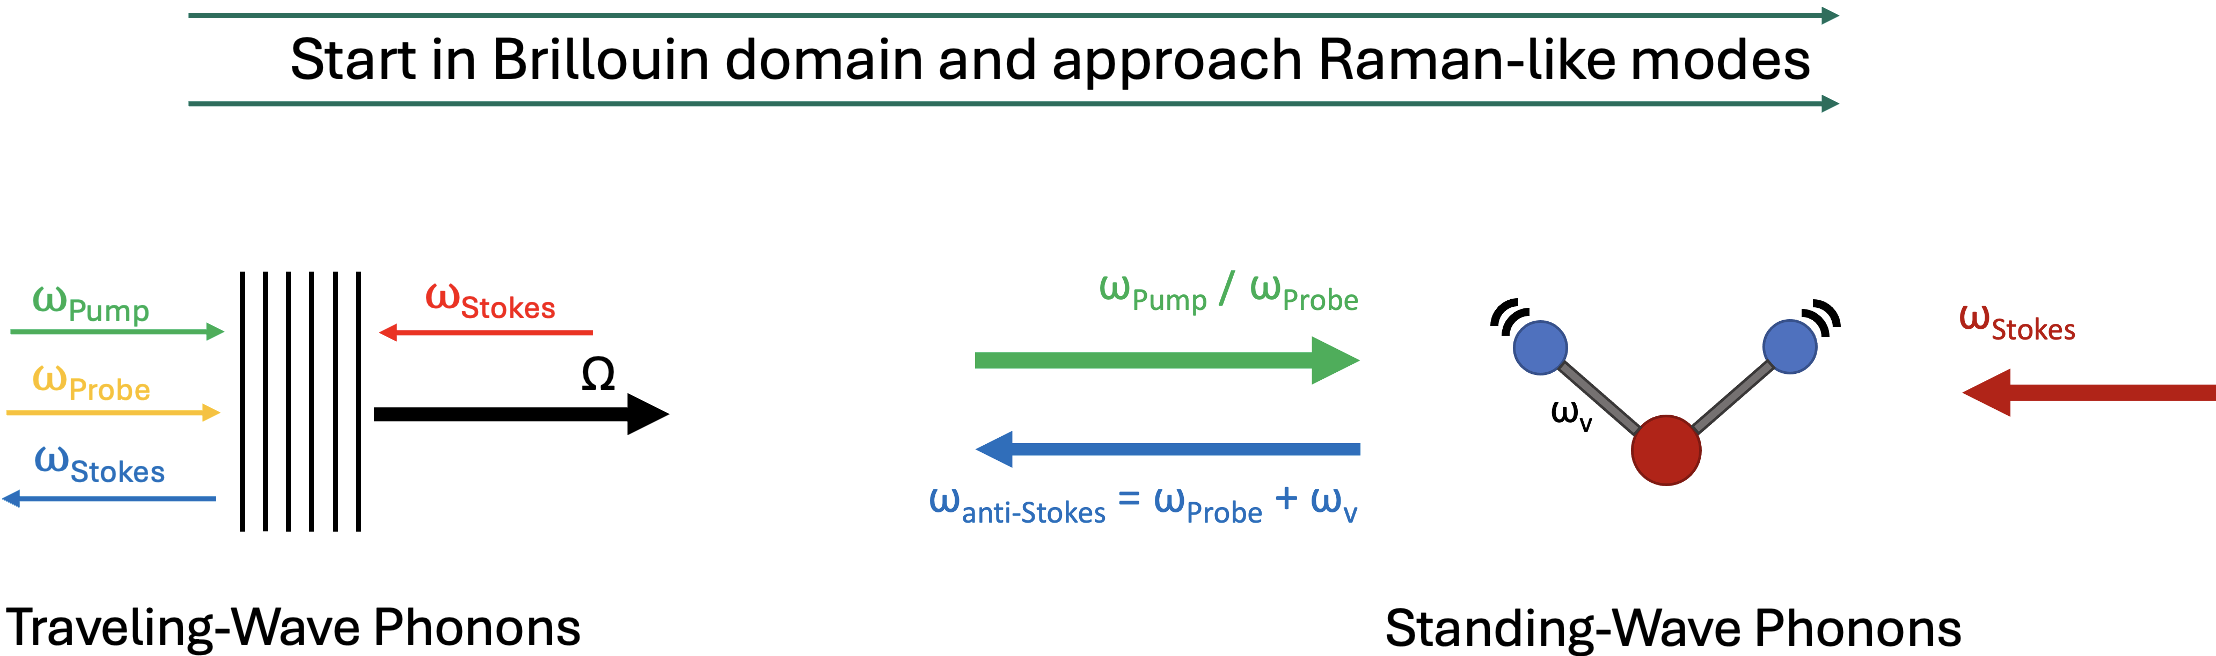
\includegraphics[width=\textwidth]{figs/4-Raman/ExploreBrillouinRamanTransition.png}
  \caption{Transition from Brillouin domain to Raman-like modes.}
  \label{fig:Raman:BrillouinRamanTransition}
\end{figure}

\begin{figure}[t]
  \centering
  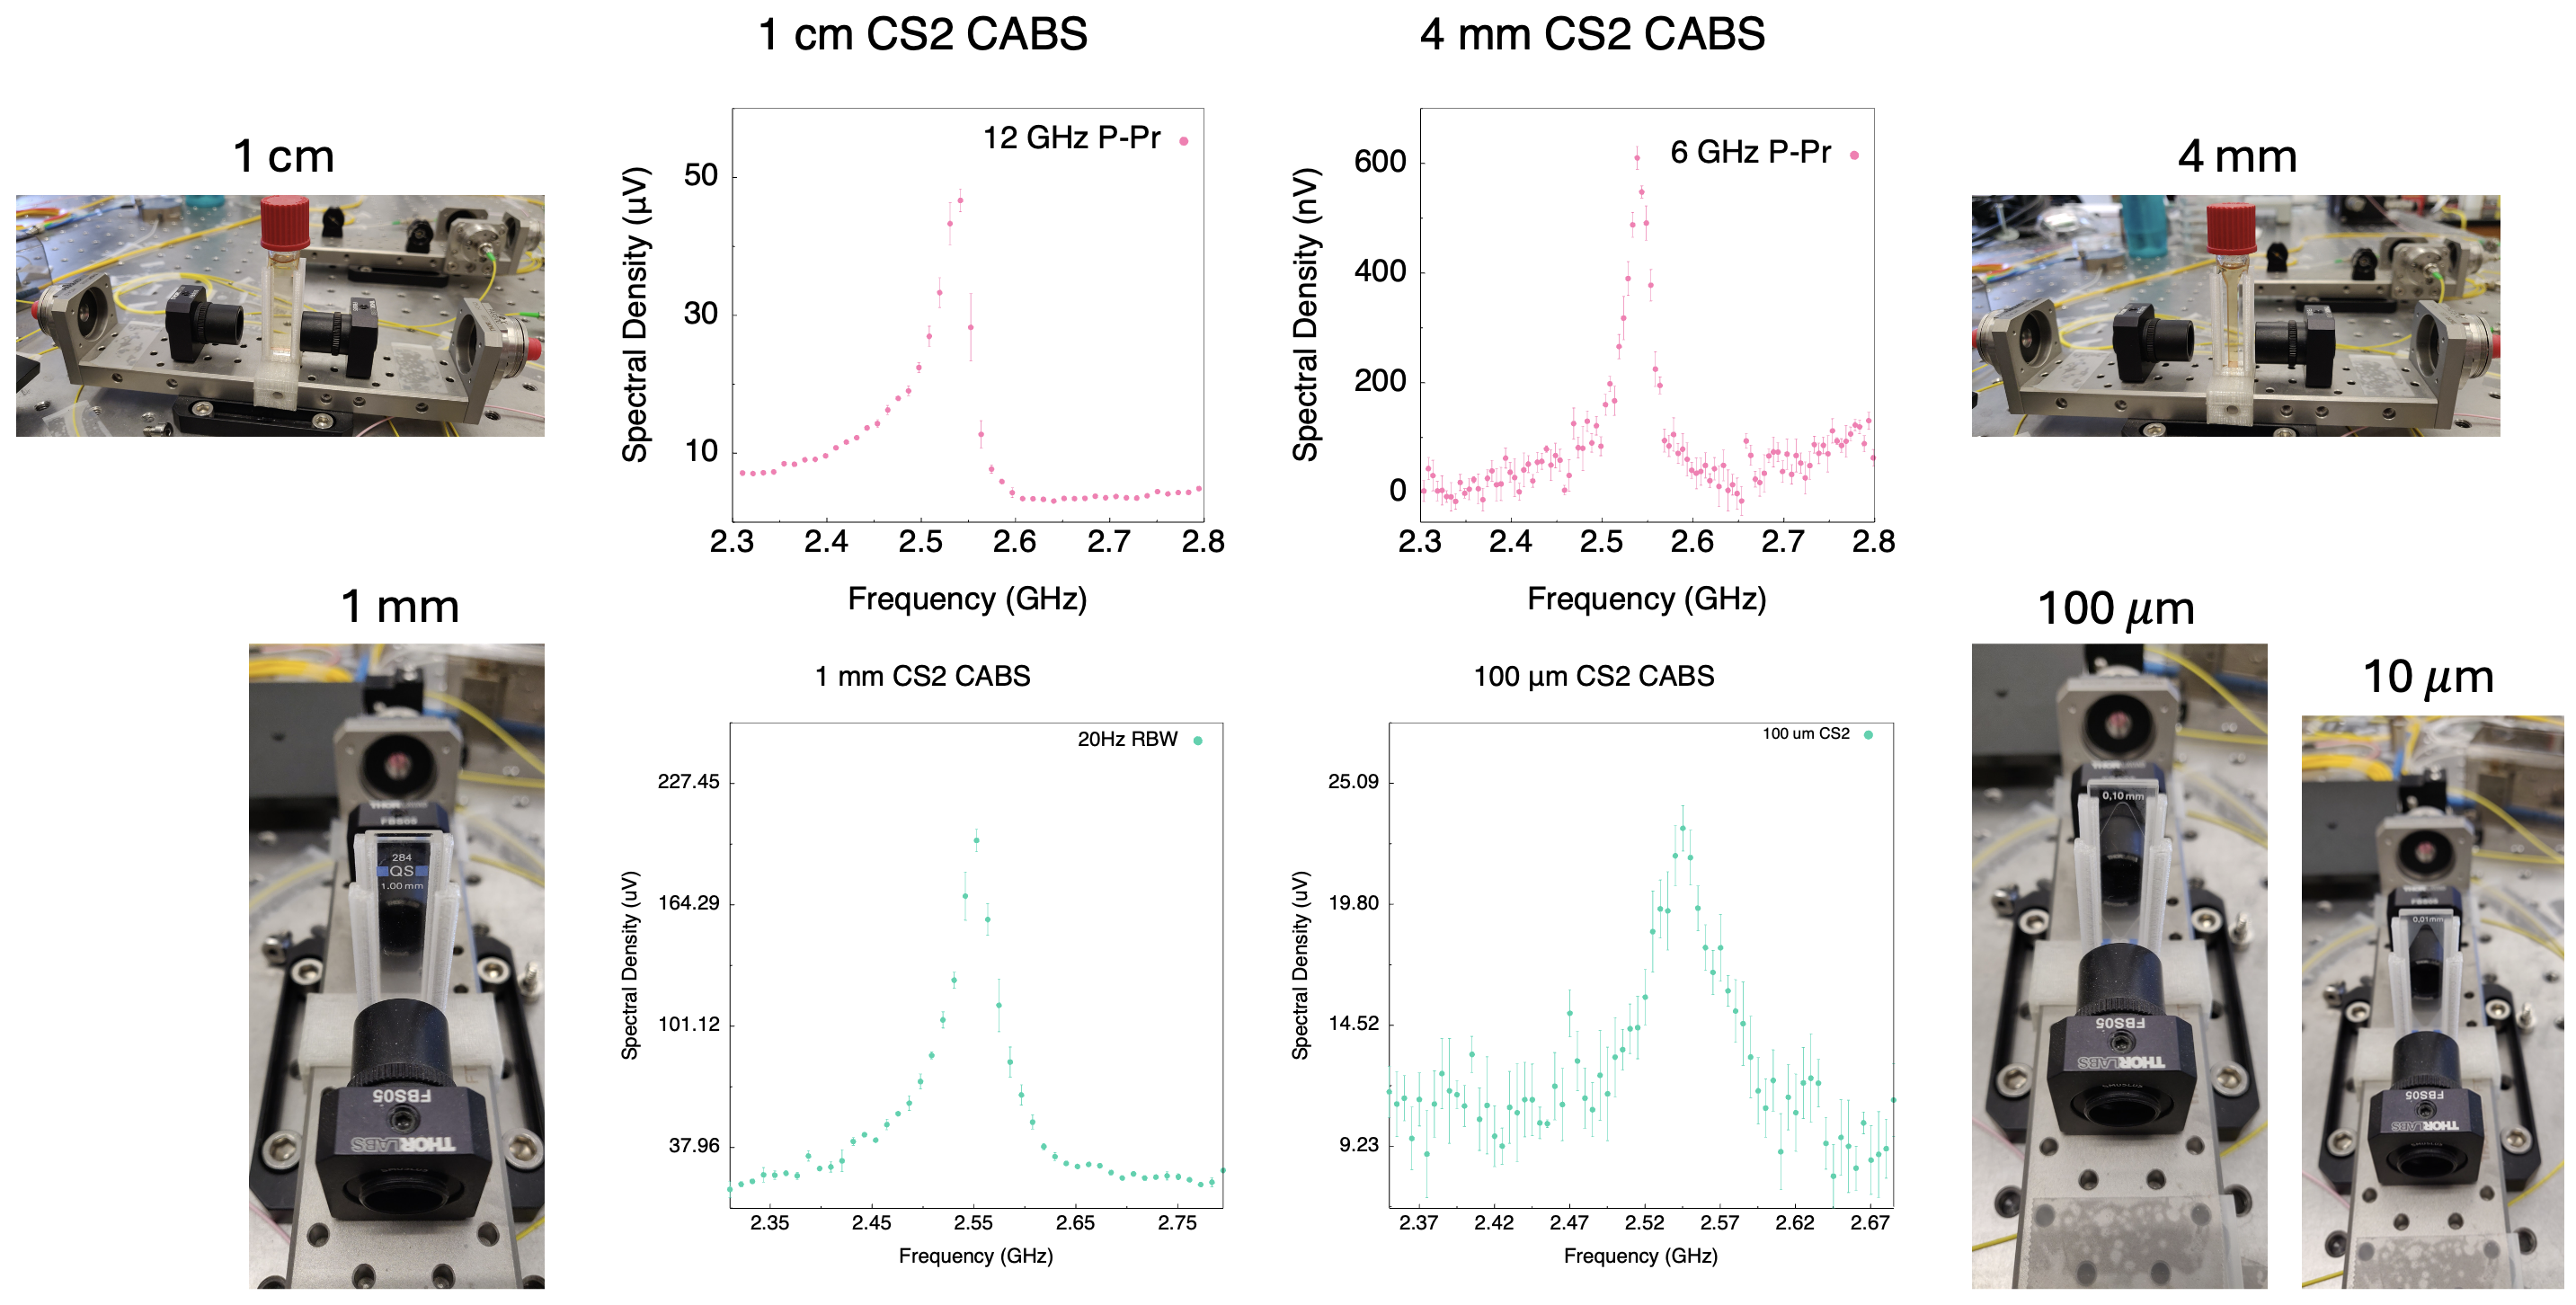
\includegraphics[width=\textwidth]{figs/4-Raman/StartBigApproachSmall.png}
  \caption{Start big, approach small.}
  \label{fig:StartBigApproachSmall}
\end{figure}

\begin{figure}[t]
  \centering
  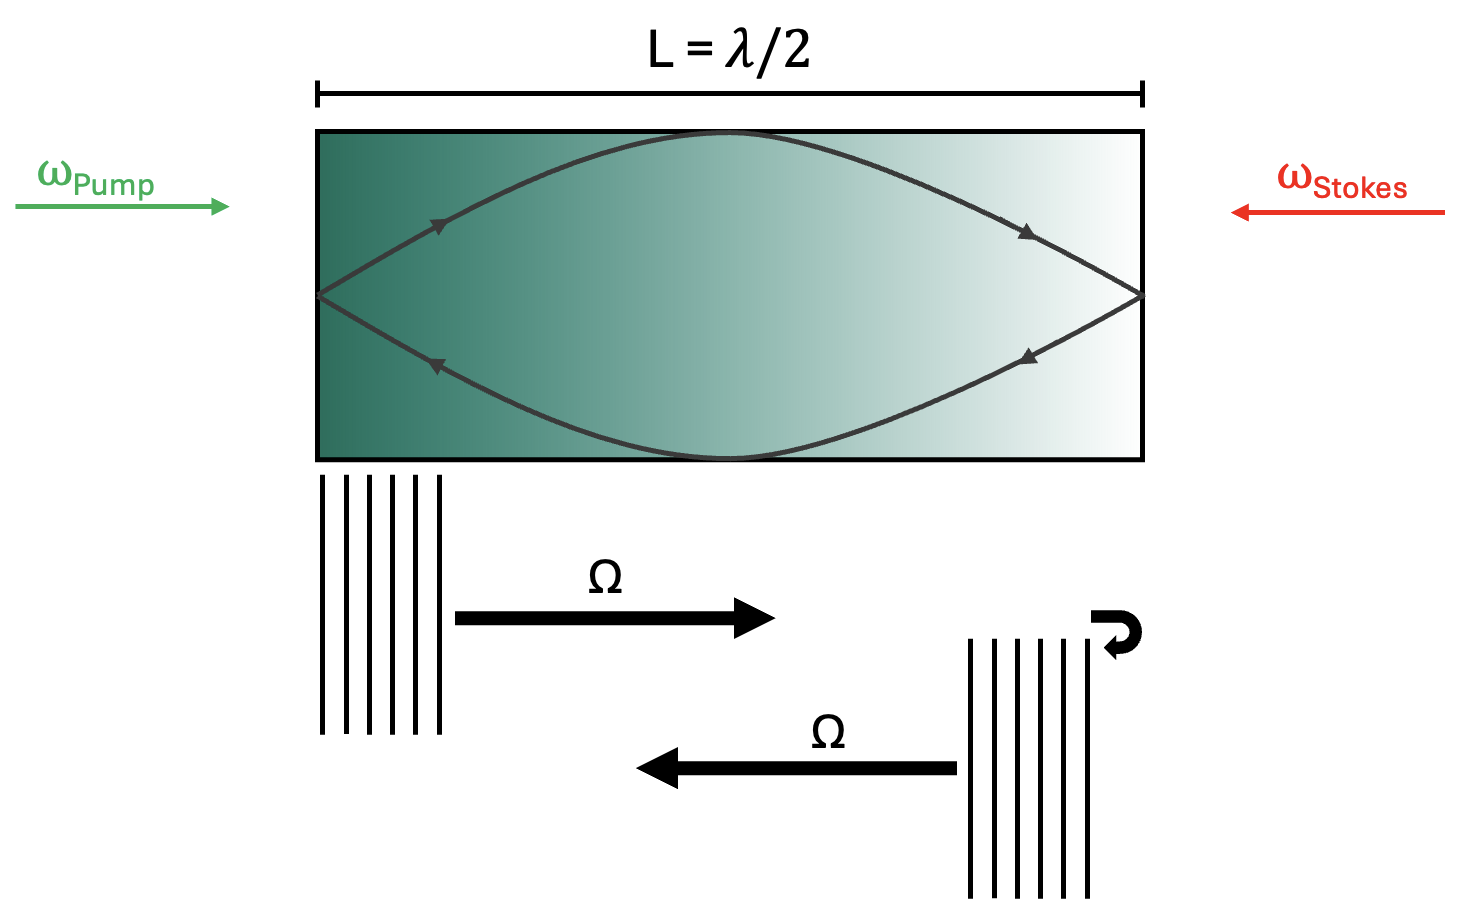
\includegraphics[width=.85\textwidth]{figs/4-Raman/GeometryDeterminesFundamentalFreq.png}
  \caption{Geometry determines fundamental frequency.}
  \label{fig:Raman:GeometryDeterminesFundamentalFreq}
\end{figure}

\subsection{Key Parameters and Feasibility}
\label{subsec:Raman:KeyParametersandFeasibility}

\begin{itemize}
  \item Describe optoacoustic response of materials (Brilluin gain coefficient \(g_{0}\), effective Brillouin gain factor \(G_{B}\) for free-space beam waist).
  \item Highlight acoustic reflection requirements: high impedance mismatch at interfaces.
  \item Summarize length-scale calculations for traveling-wave phonons to become standing waves, factoring in acoustic attenuation length and boundary conditions. (Mean phonon travel distance based on sound speed and dissipation rate)
\end{itemize}

\begin{figure}[t]
  \centering
  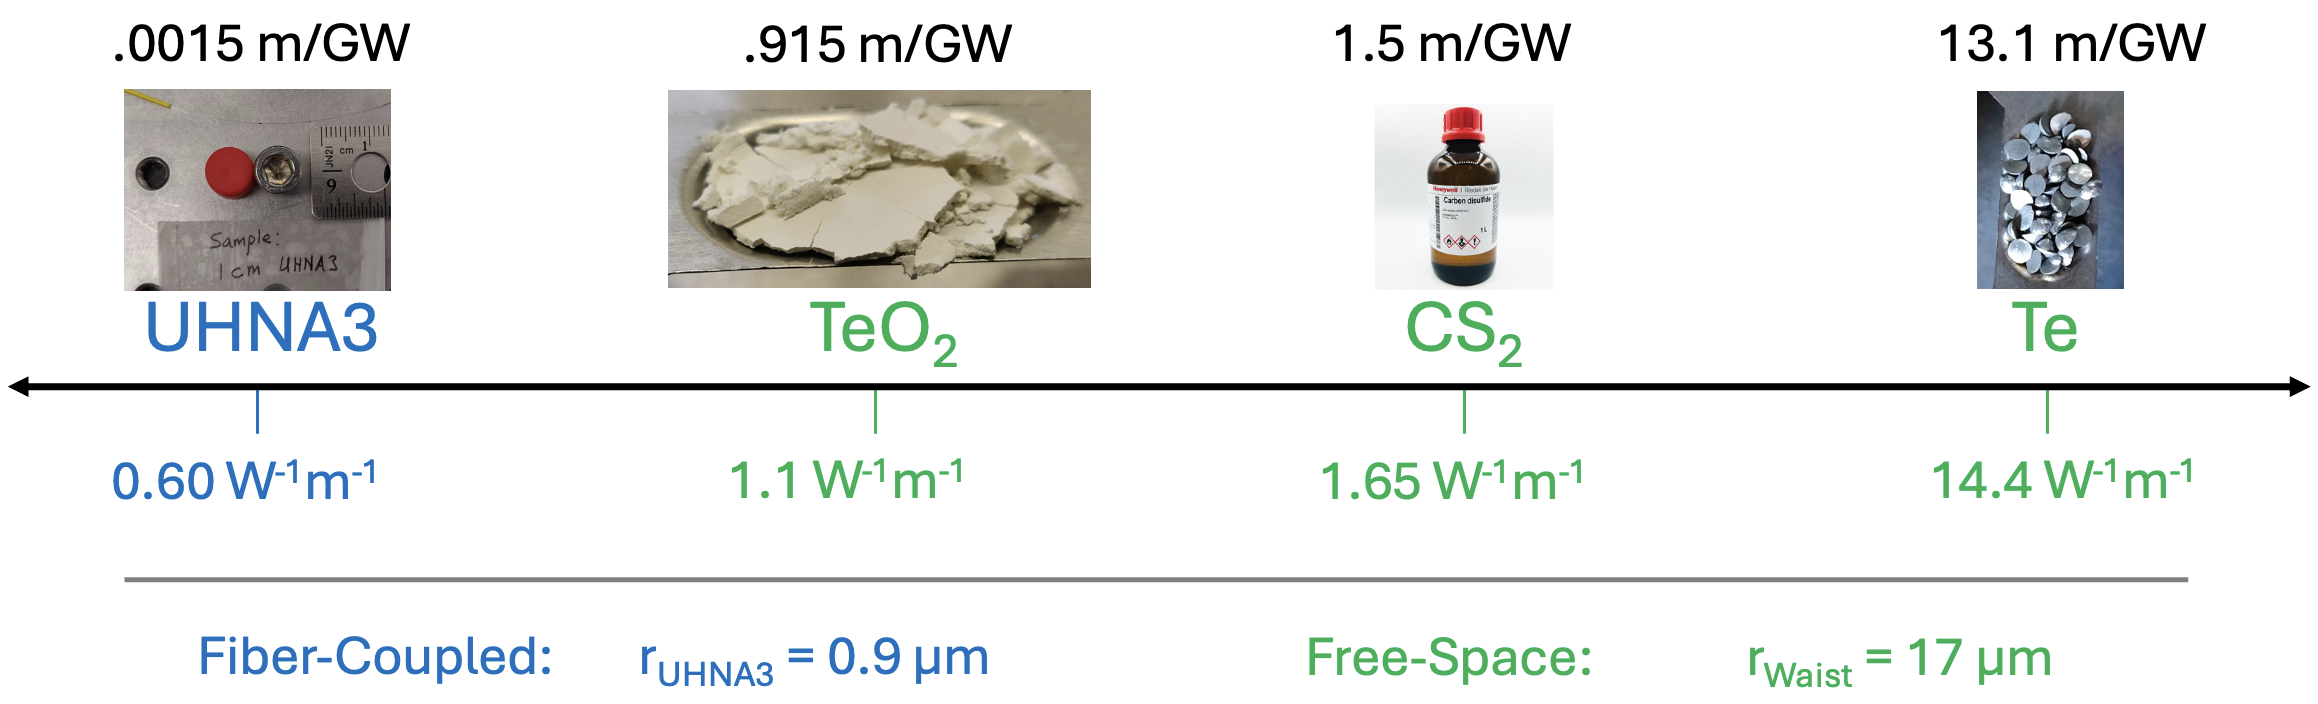
\includegraphics[width=\textwidth]{figs/4-Raman/GainOfRelevantMaterials.png}
  \caption{Gain of relevant materials.}
  \label{fig:Raman:GainOfRelevantMaterials}
\end{figure}

\begin{figure}[t]
  \centering
  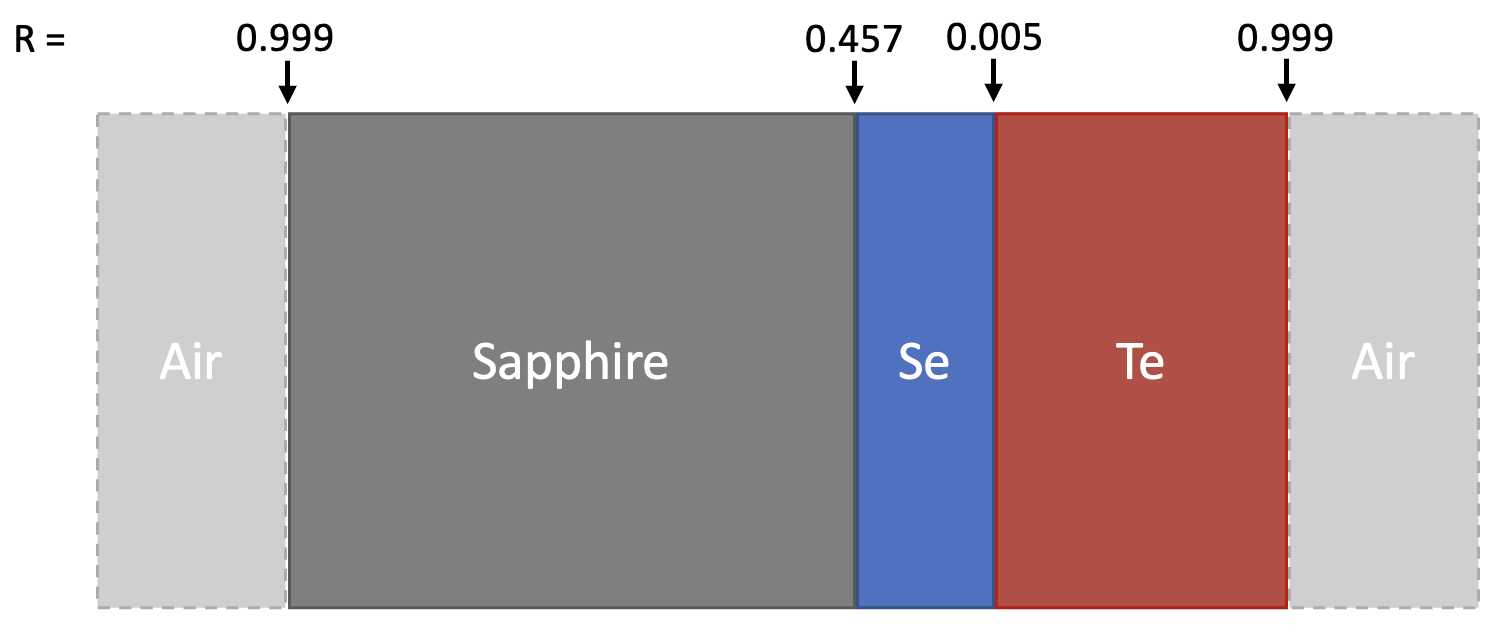
\includegraphics[width=\textwidth]{figs/4-Raman/AcousticImpedance.png}
  \caption{Acoustic impedance.}
  \label{fig:Raman:AcousticImpedance}
\end{figure}

%--------------------------------------------------------------------%

\section{Experimental Platforms and Collaborative Fabrication}
\label{sec:Raman:ExperimentalPlatformsandCollaborativeFabrication}

\subsection{Germanium-Doped Optical Fiber}
\label{subsec:Raman:Target:UHNA3}

1cm -> 1mm

\begin{figure}[t]
    \centering
    \begin{subfigure}[b]{0.49\textwidth}
        \centering
        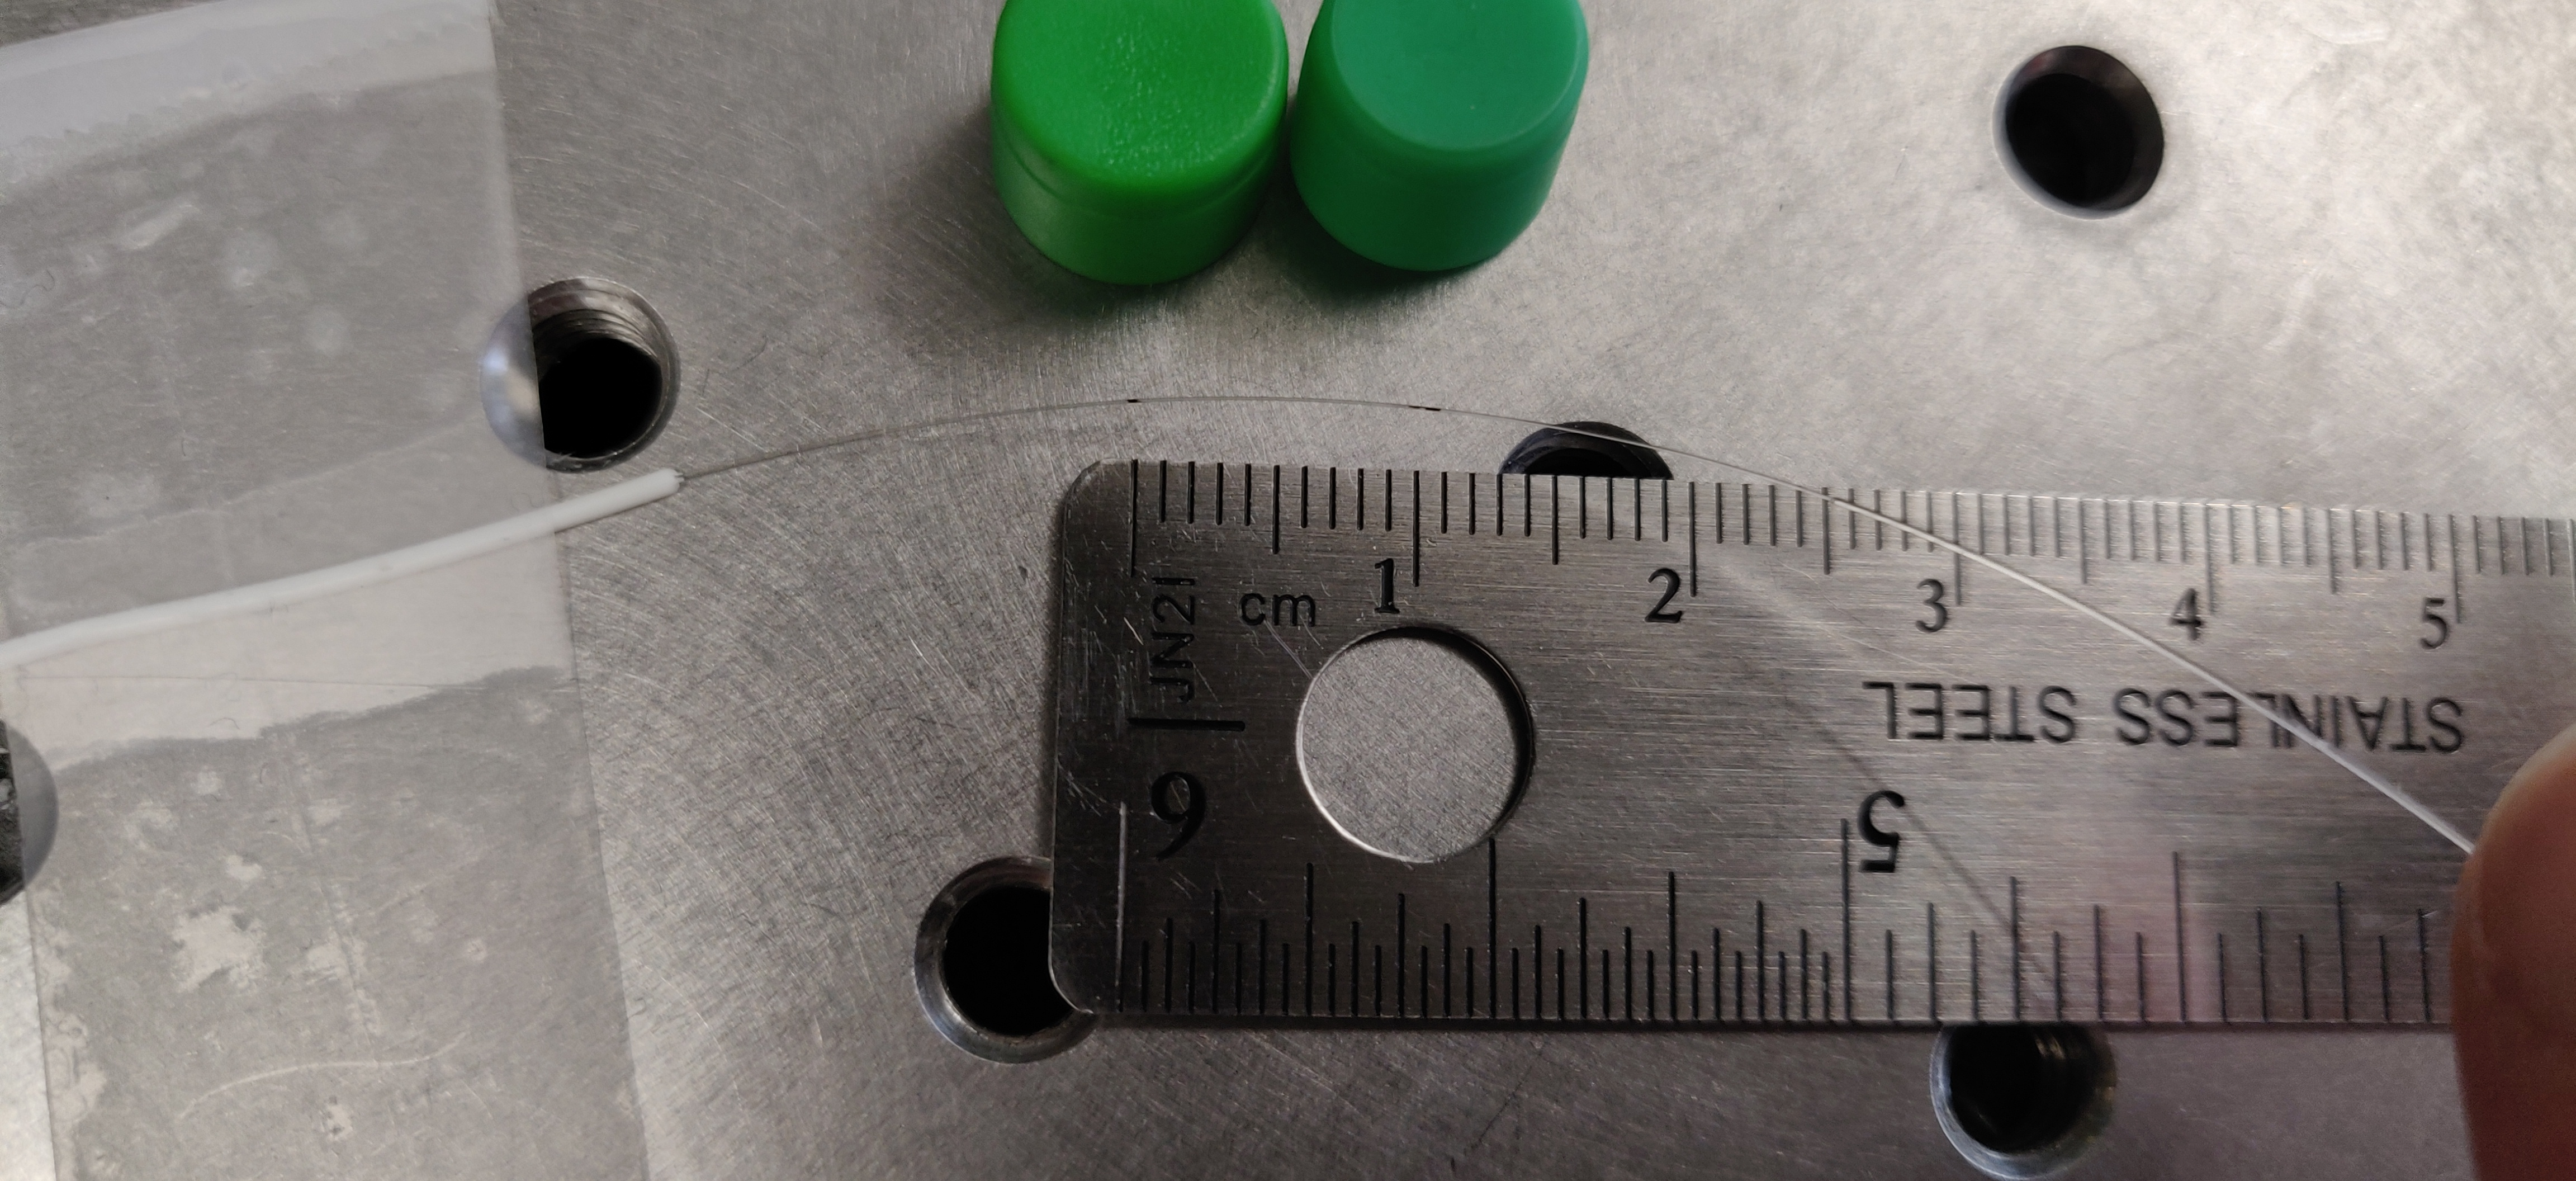
\includegraphics[width=\textwidth]{figs/4-Raman/1cm UHNA3.jpeg}
        \caption{}
        \label{fig:Raman:1cmUHNA3pic}
    \end{subfigure}
    \hfill
    \begin{subfigure}[b]{0.49\textwidth}
        \centering
        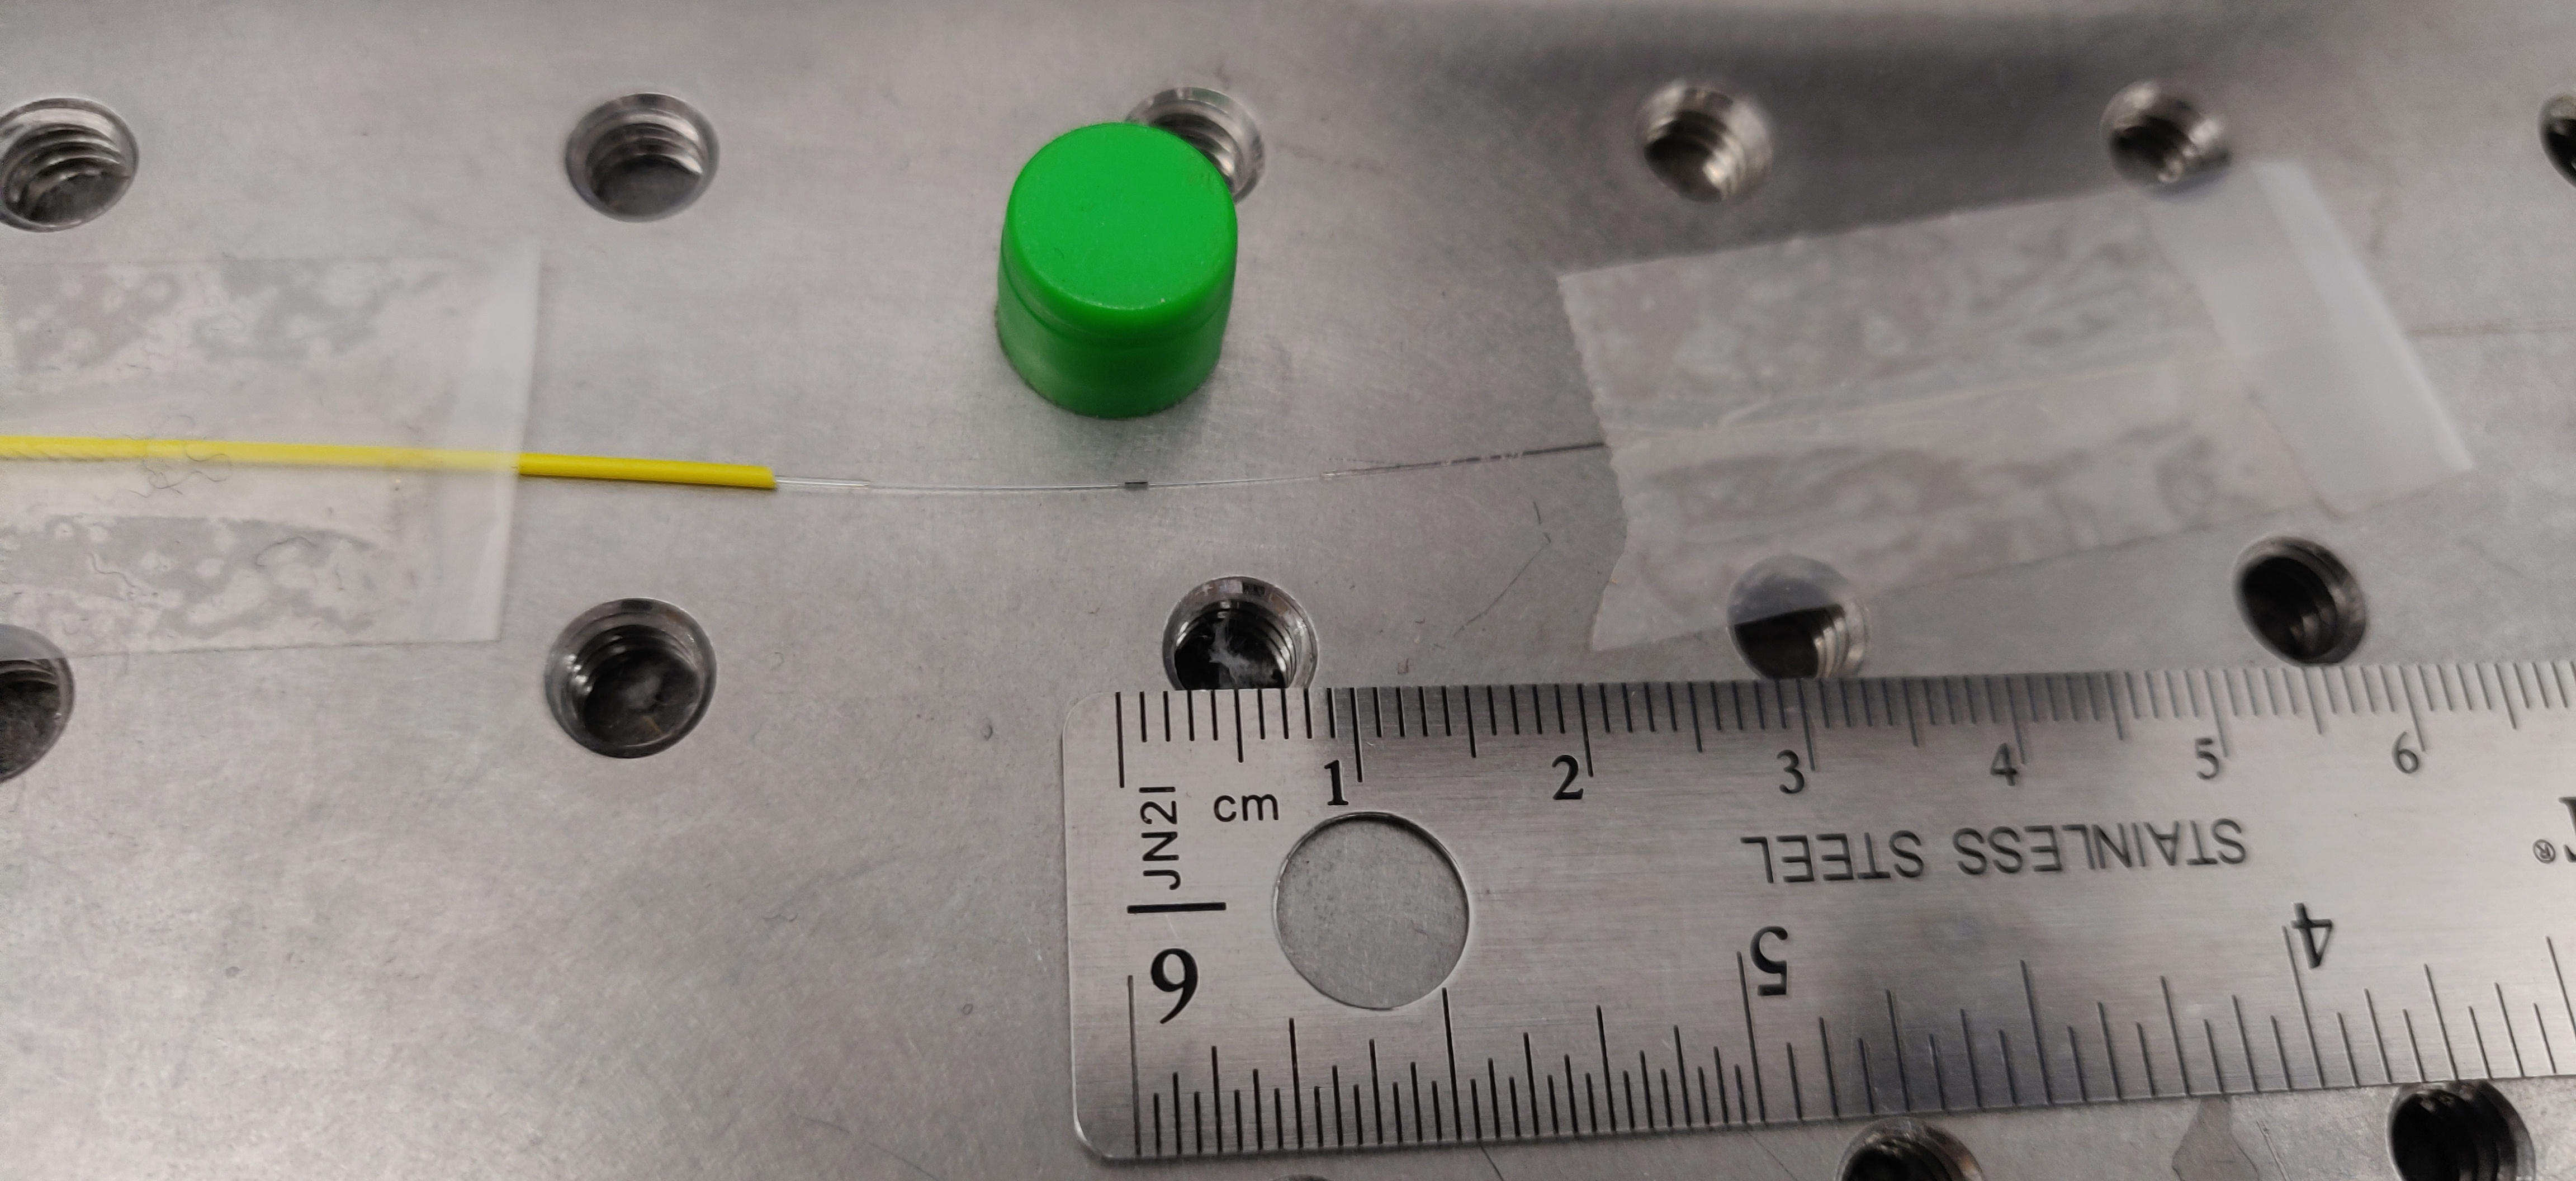
\includegraphics[width=\textwidth]{figs/4-Raman/1mm UHNA3 in apparatus.jpeg}
        \caption{}
        \label{fig:Raman:1mmUHNA3pic}
    \end{subfigure}
    \caption{\SI{1}{\centi\meter} (\ref{fig:Raman:1cmUHNA3pic}) and \SI{1}{\milli\meter} (\ref{fig:Raman:1mmUHNA3pic}) \ac{UHNA3}.}
    \label{fig:Raman:UHNA3}
\end{figure}

\subsection{Free-Space Optics with Liquid Carbon Disulfide}
\label{subsec:Raman:Target:CS2Vial}

Free space with vial

\begin{figure}[t]
    \centering
    \begin{subfigure}[b]{0.49\textwidth}
        \centering
        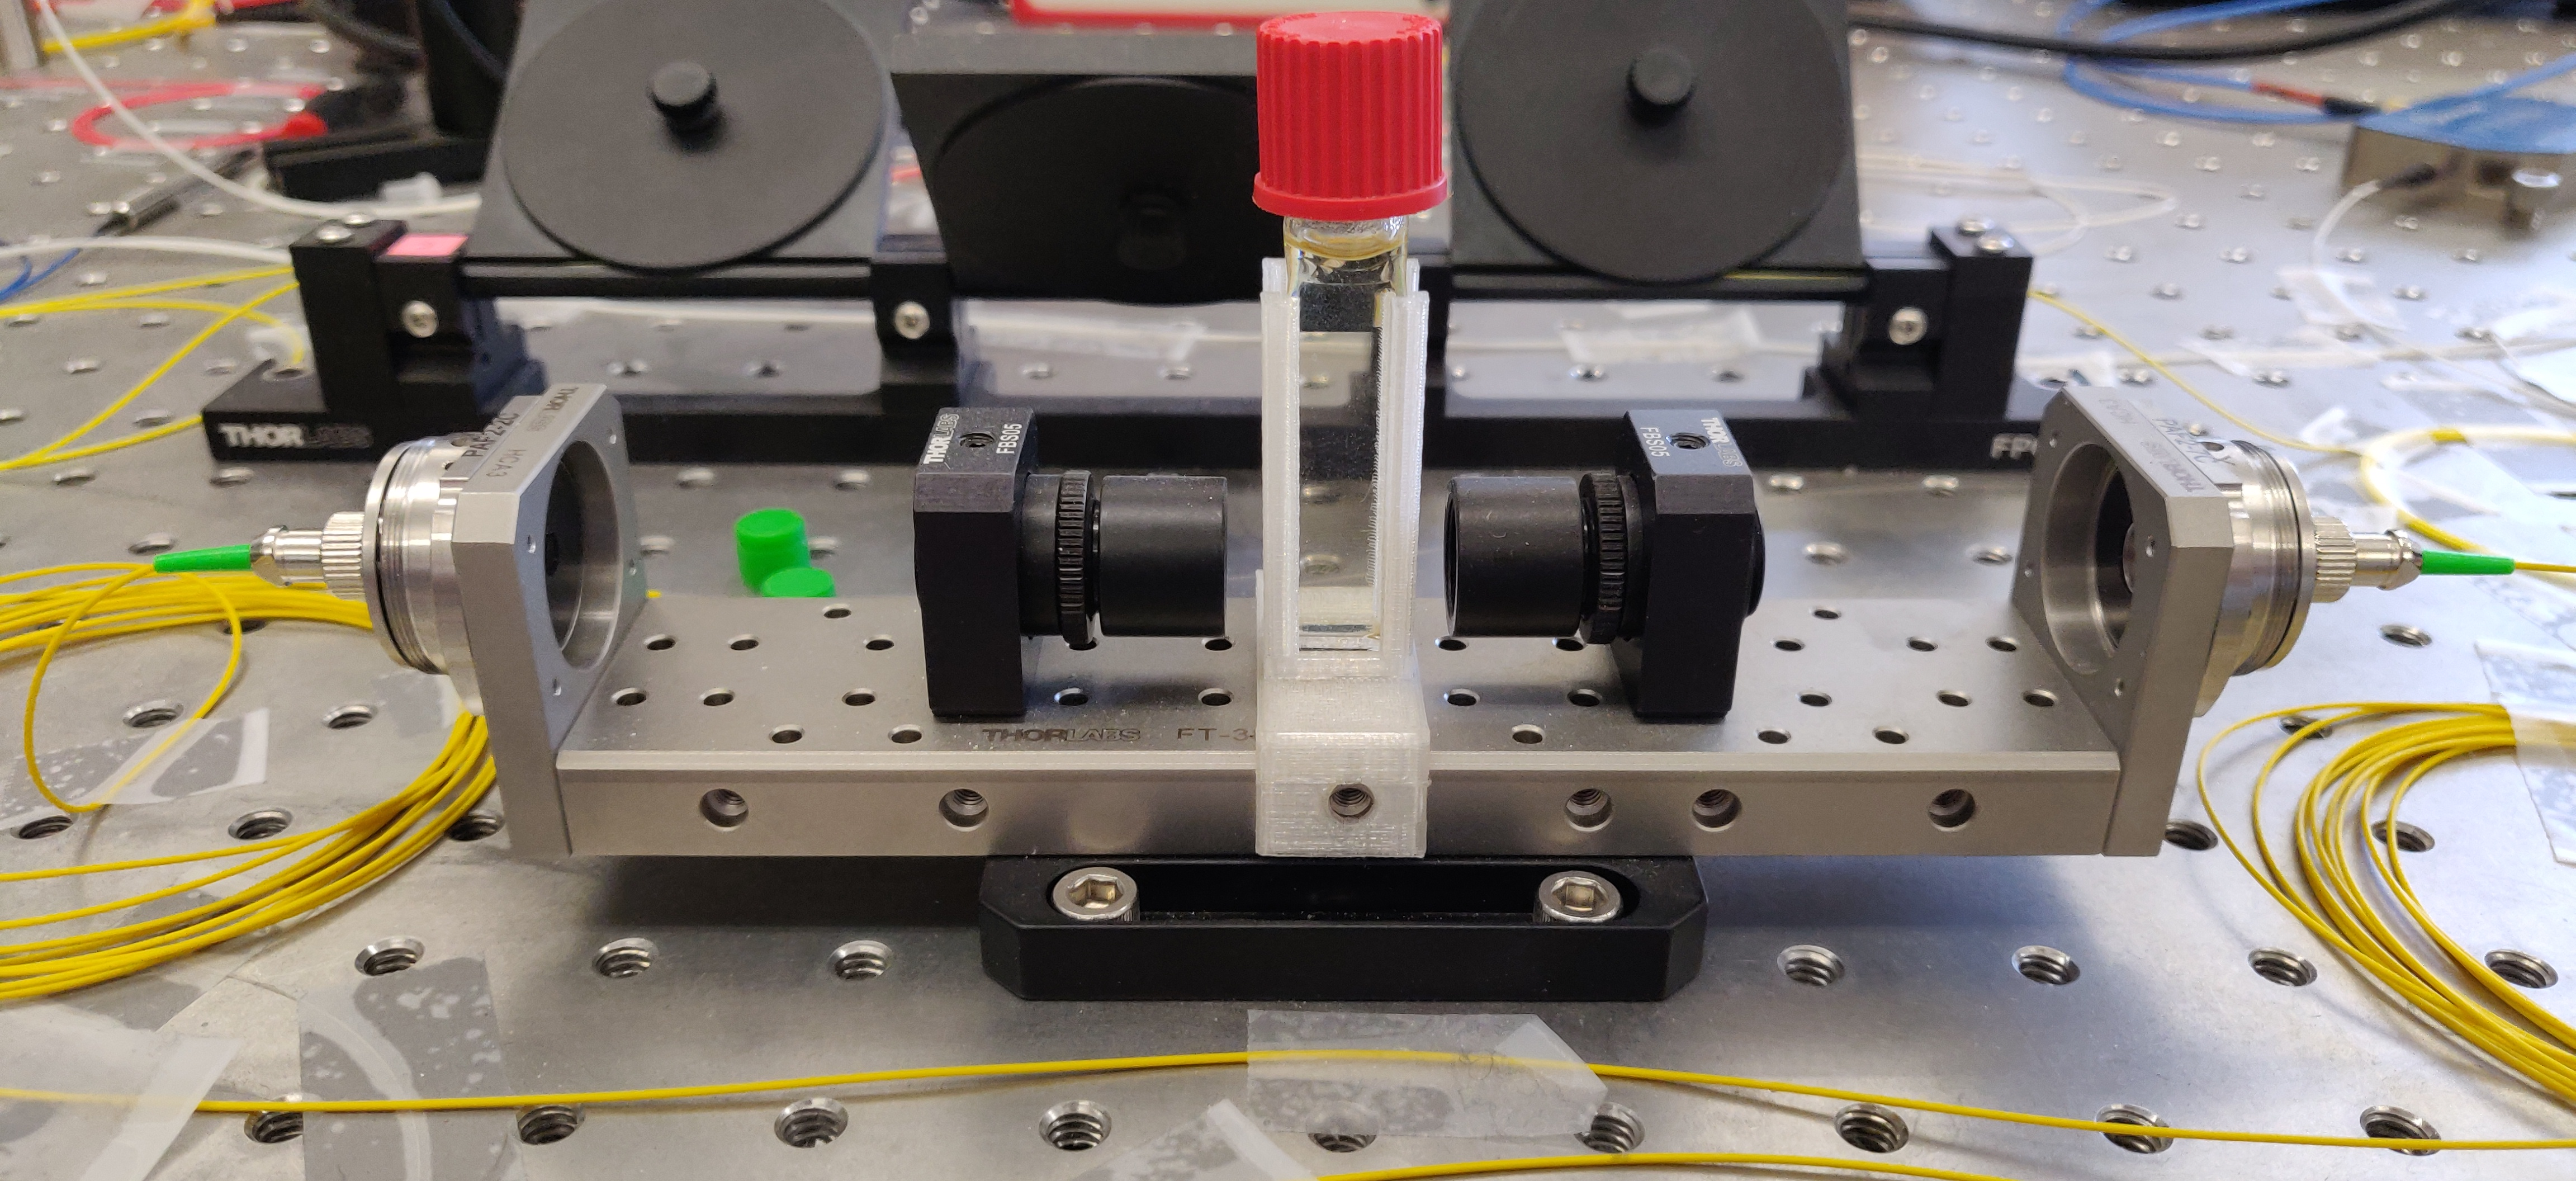
\includegraphics[width=\textwidth]{figs/4-Raman/1cmCS2.jpeg}
        \caption{}
        \label{fig:Raman:1cmCS2}
    \end{subfigure}
    \hfill
    \begin{subfigure}[b]{0.49\textwidth}
        \centering
        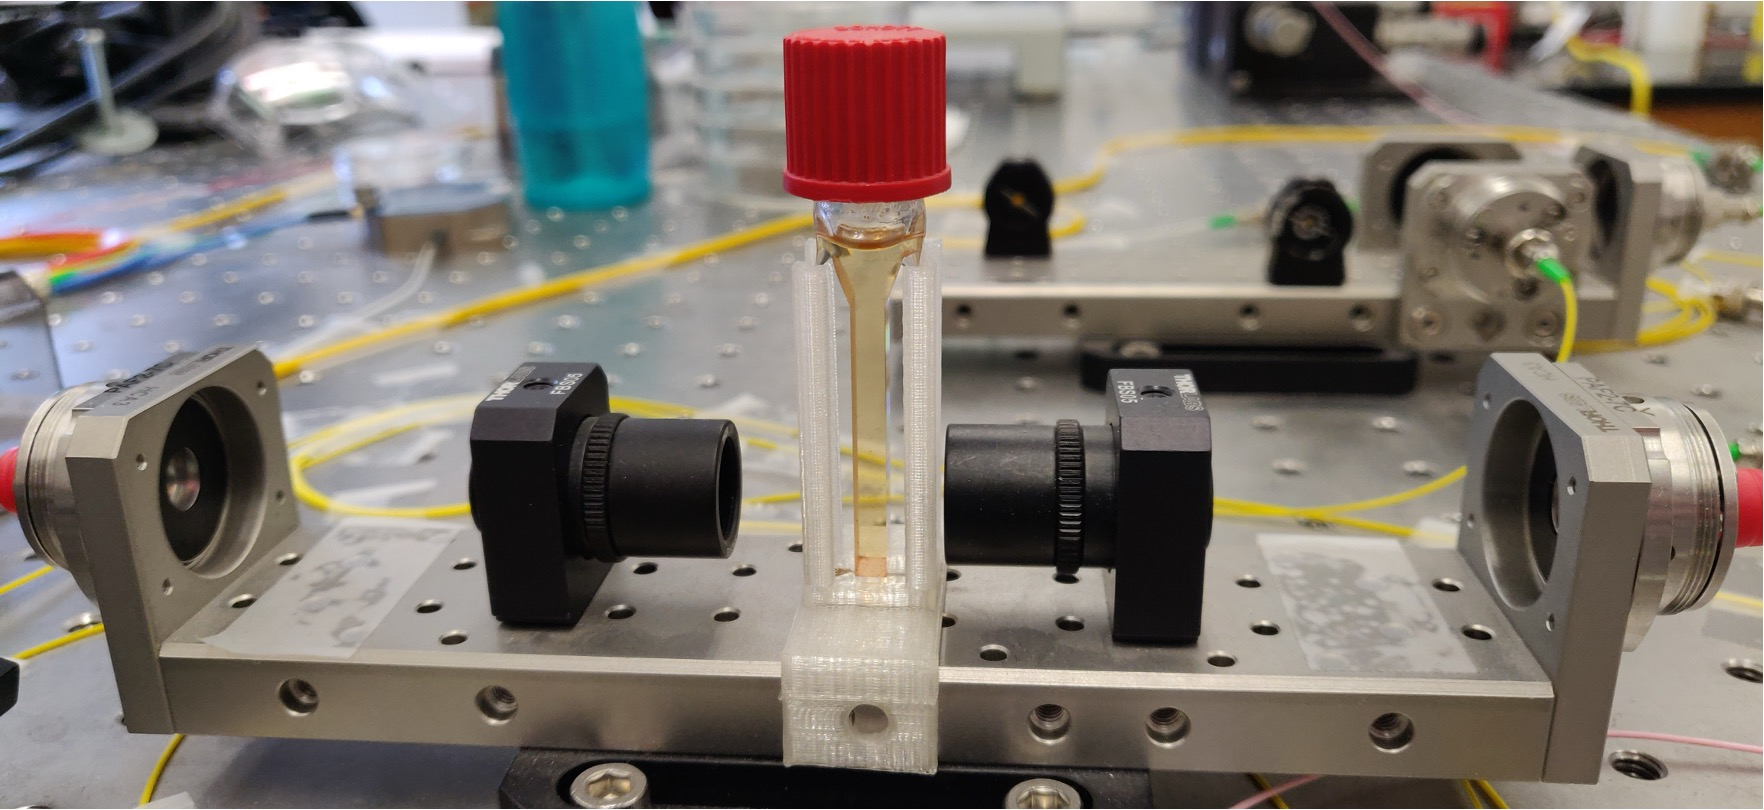
\includegraphics[width=\textwidth]{figs/4-Raman/4mmCS2.jpg}
        \caption{}
        \label{fig:Raman:4mmCS2}
    \end{subfigure}
    \caption{\SI{1}{\centi\meter} (\ref{fig:Raman:1cmCS2}) and \SI{4}{\milli\meter} (\ref{fig:Raman:4mmCS2}) liquid \ce{CS2}.}
    \label{fig:Raman:CS2Cuvet}
\end{figure}

\subsection{Tellurium Dioxide Thin Film}
\label{subsec:Raman:Target:TeO2}

Gibbs collab
deposit Te, oxidize into TeO2

table of relevant TeO2 parameters

\subsection{Tellurium Thin Film}
\label{subsec:Raman:Target:Te}

Gibbs collab and CINT collab
oxidizes to TeO2

table of relevant Te parameters

\subsection{Carbon Disulfide Micrometer Cell}
\label{subsec:Raman:Target:CS2Cells}

table of relevant CS2 parameters

cells -> 1 W amp, bubble test

\begin{figure}[t]
  \centering
  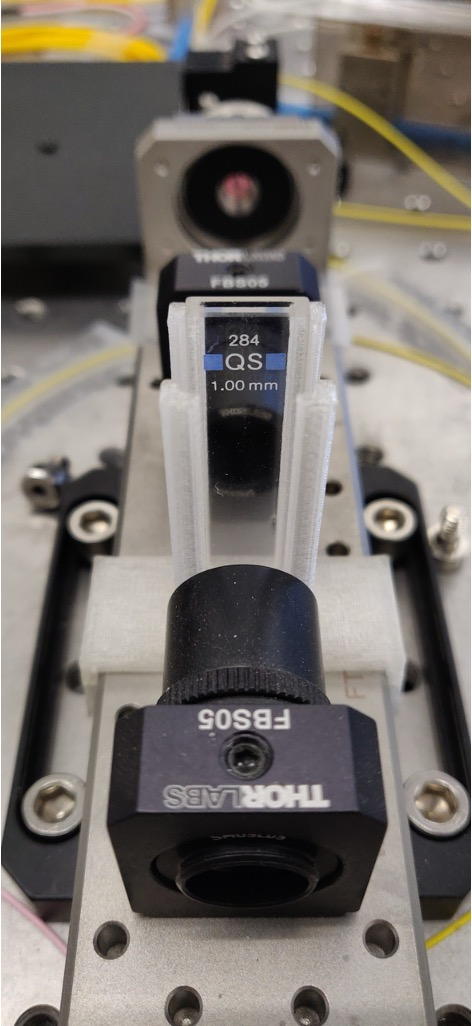
\includegraphics[width=\textwidth]{figs/4-Raman/1mmCS2.jpg}
  \caption{\SI{1}{\milli\meter} \ce{CS2} cell secured in beam path of \acl{CoBS}.}
  \label{fig:Raman:1mmCS2}
\end{figure}

\begin{figure}[t]
  \centering
  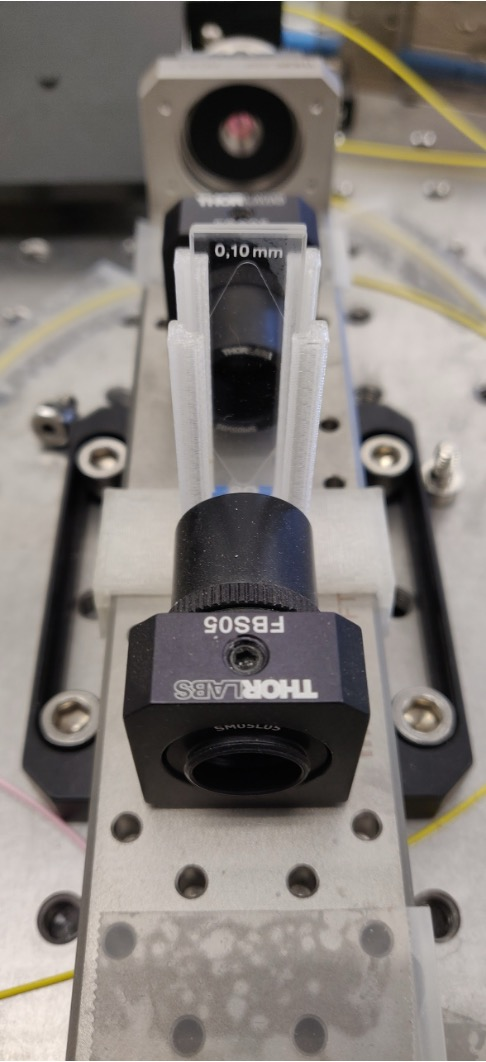
\includegraphics[width=\textwidth]{figs/4-Raman/100umCS2.jpg}
  \caption{\SI{100}{\micro\meter} \ce{CS2} cell secured in beam path of \acl{CoBS}.}
  \label{fig:Raman:100umCS2}
\end{figure}

\begin{figure}[t]
  \centering
  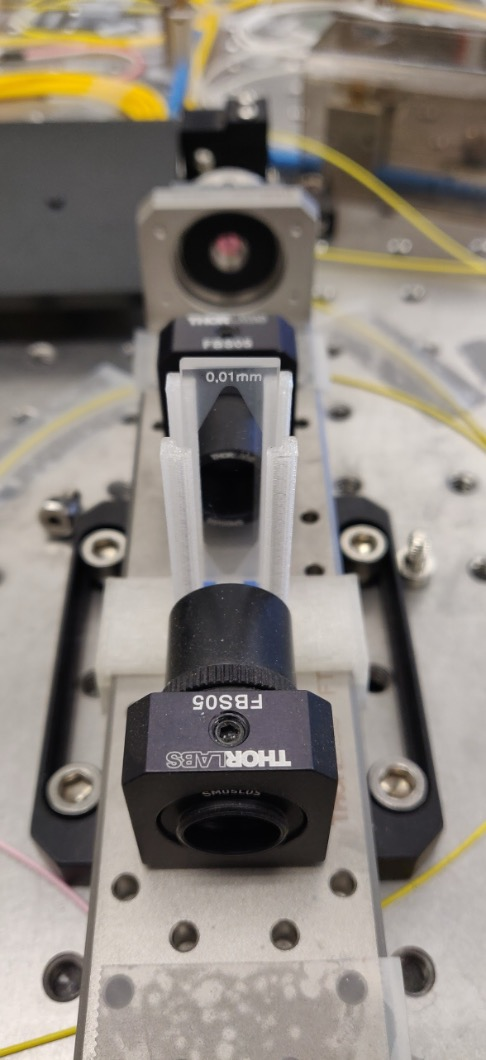
\includegraphics[width=\textwidth]{figs/4-Raman/10umCS2.jpg}
  \caption{\SI{10}{\micro\meter} \ce{CS2} cell secured in beam path of \acl{CoBS}.}
  \label{fig:Raman:10umCS2}
\end{figure}

\subsection{Suspended Silica Rib Waveguide}
\label{subsec:Raman:Target:Waveguide}

BYU collab
If we can couple chip waveguide into CoBS fiber-chip-fiber, then we have access to a playground of materials and geometries
initial test took 9 months to learn and measure


\subsection{Elastically-Suspended Photonic-Phononic Waveguide}
\label{subsec:Raman:Target:WigglyWaveguide}

BYU collab
proof of fabrication: holes and trampoline

%--------------------------------------------------------------------%

\section{Methods}
\label{sec:Raman:Methods}

\subsection{Instrument Overview}
\label{subsec:Raman:InstrumentOverview}

\begin{itemize}
  \item Recap the Coherently Stimulated Brillouin Spectrometer from Chapter 3, emphasizing its high sensitivity and relaxed phase-matching.
  \item Note additional improvements or calibration steps performed for these particular experiments.
\end{itemize}

\subsection{Measurement Protocol}
\label{subsec:Raman:MeasurementProtocol}

\begin{itemize}
  \item Walk through how pump and probe fields are injected into the samples (liquid cells, waveguides, films).
  \item How you monitor and collect scattered light at/near the expected Brillouin frequency, watching for discrete or multi-peak features.
  \item Typical data-acquisition settings (power ranges, frequency scans, detection bandwidth, etc.).
\end{itemize}

\subsection{Data Analysis Steps}
\label{subsec:Raman:DataAnalysisSteps}

\begin{itemize}
  \item Call back to Lorentzian versus Fano-shape fitting for small signals
  \item Mention Lorentzian versus multi-peak fitting to identify discrete modes.
  \item Emphasize strategies to distinguish genuine signals from instrument background, referencing instrument artifacts discovered previously.
  \item Summarize how you accounted for temperature effects, boundary reflections, or chemical transformations (like Te to TeO\textsubscript{2}).
\end{itemize}

%--------------------------------------------------------------------%

\section{Results}
\label{sec:Raman:Results}

UHNA3 - 1cm, 1mm
CS2 vial - 4mm, 2mm
TeO2 films - 1um, 500nm
CS2 - 1mm, 100um, (10um not quite)
chip waveguide - chip/nochip, holes

\subsection{Initial Findings}
\label{subsec:Raman:InitialFindings}

\begin{itemize}
  \item Display earliest data (e.g., on Te thin films) and how a strong feature turned out to be electronic background.
  \item Show subsequent measurements (CS\textsubscript{2}, chip waveguides) and partial successes, such as spectral distortions suggesting mode splitting.
\end{itemize}

\subsection{Challenges and Partial Outcomes}
\label{subsec:Raman:ChallengesandPartialOutcomes}

\begin{itemize}
  \item Explain complexity of proving Raman-like modes: acoustic mismatch, unexpected phonon damping, oxidation/ablation of thin films, or sample delays.
  \item Highlight any improvements you achieved (e.g., 11\(\times\) scattered-signal boost) and how close you were to threshold detection.
\end{itemize}

\subsection{Interpretation in Light of Theory}
\label{subsec:Raman:InterpretationinLightofTheory}

\begin{itemize}
  \item Note which observations align with the traveling-wave to standing-wave hypothesis.
  \item Speculate on why a clear discrete Raman ladder was not definitively observed (path length, reflectivity, line broadening, etc.).
\end{itemize}

\begin{figure}[t]
  \centering
  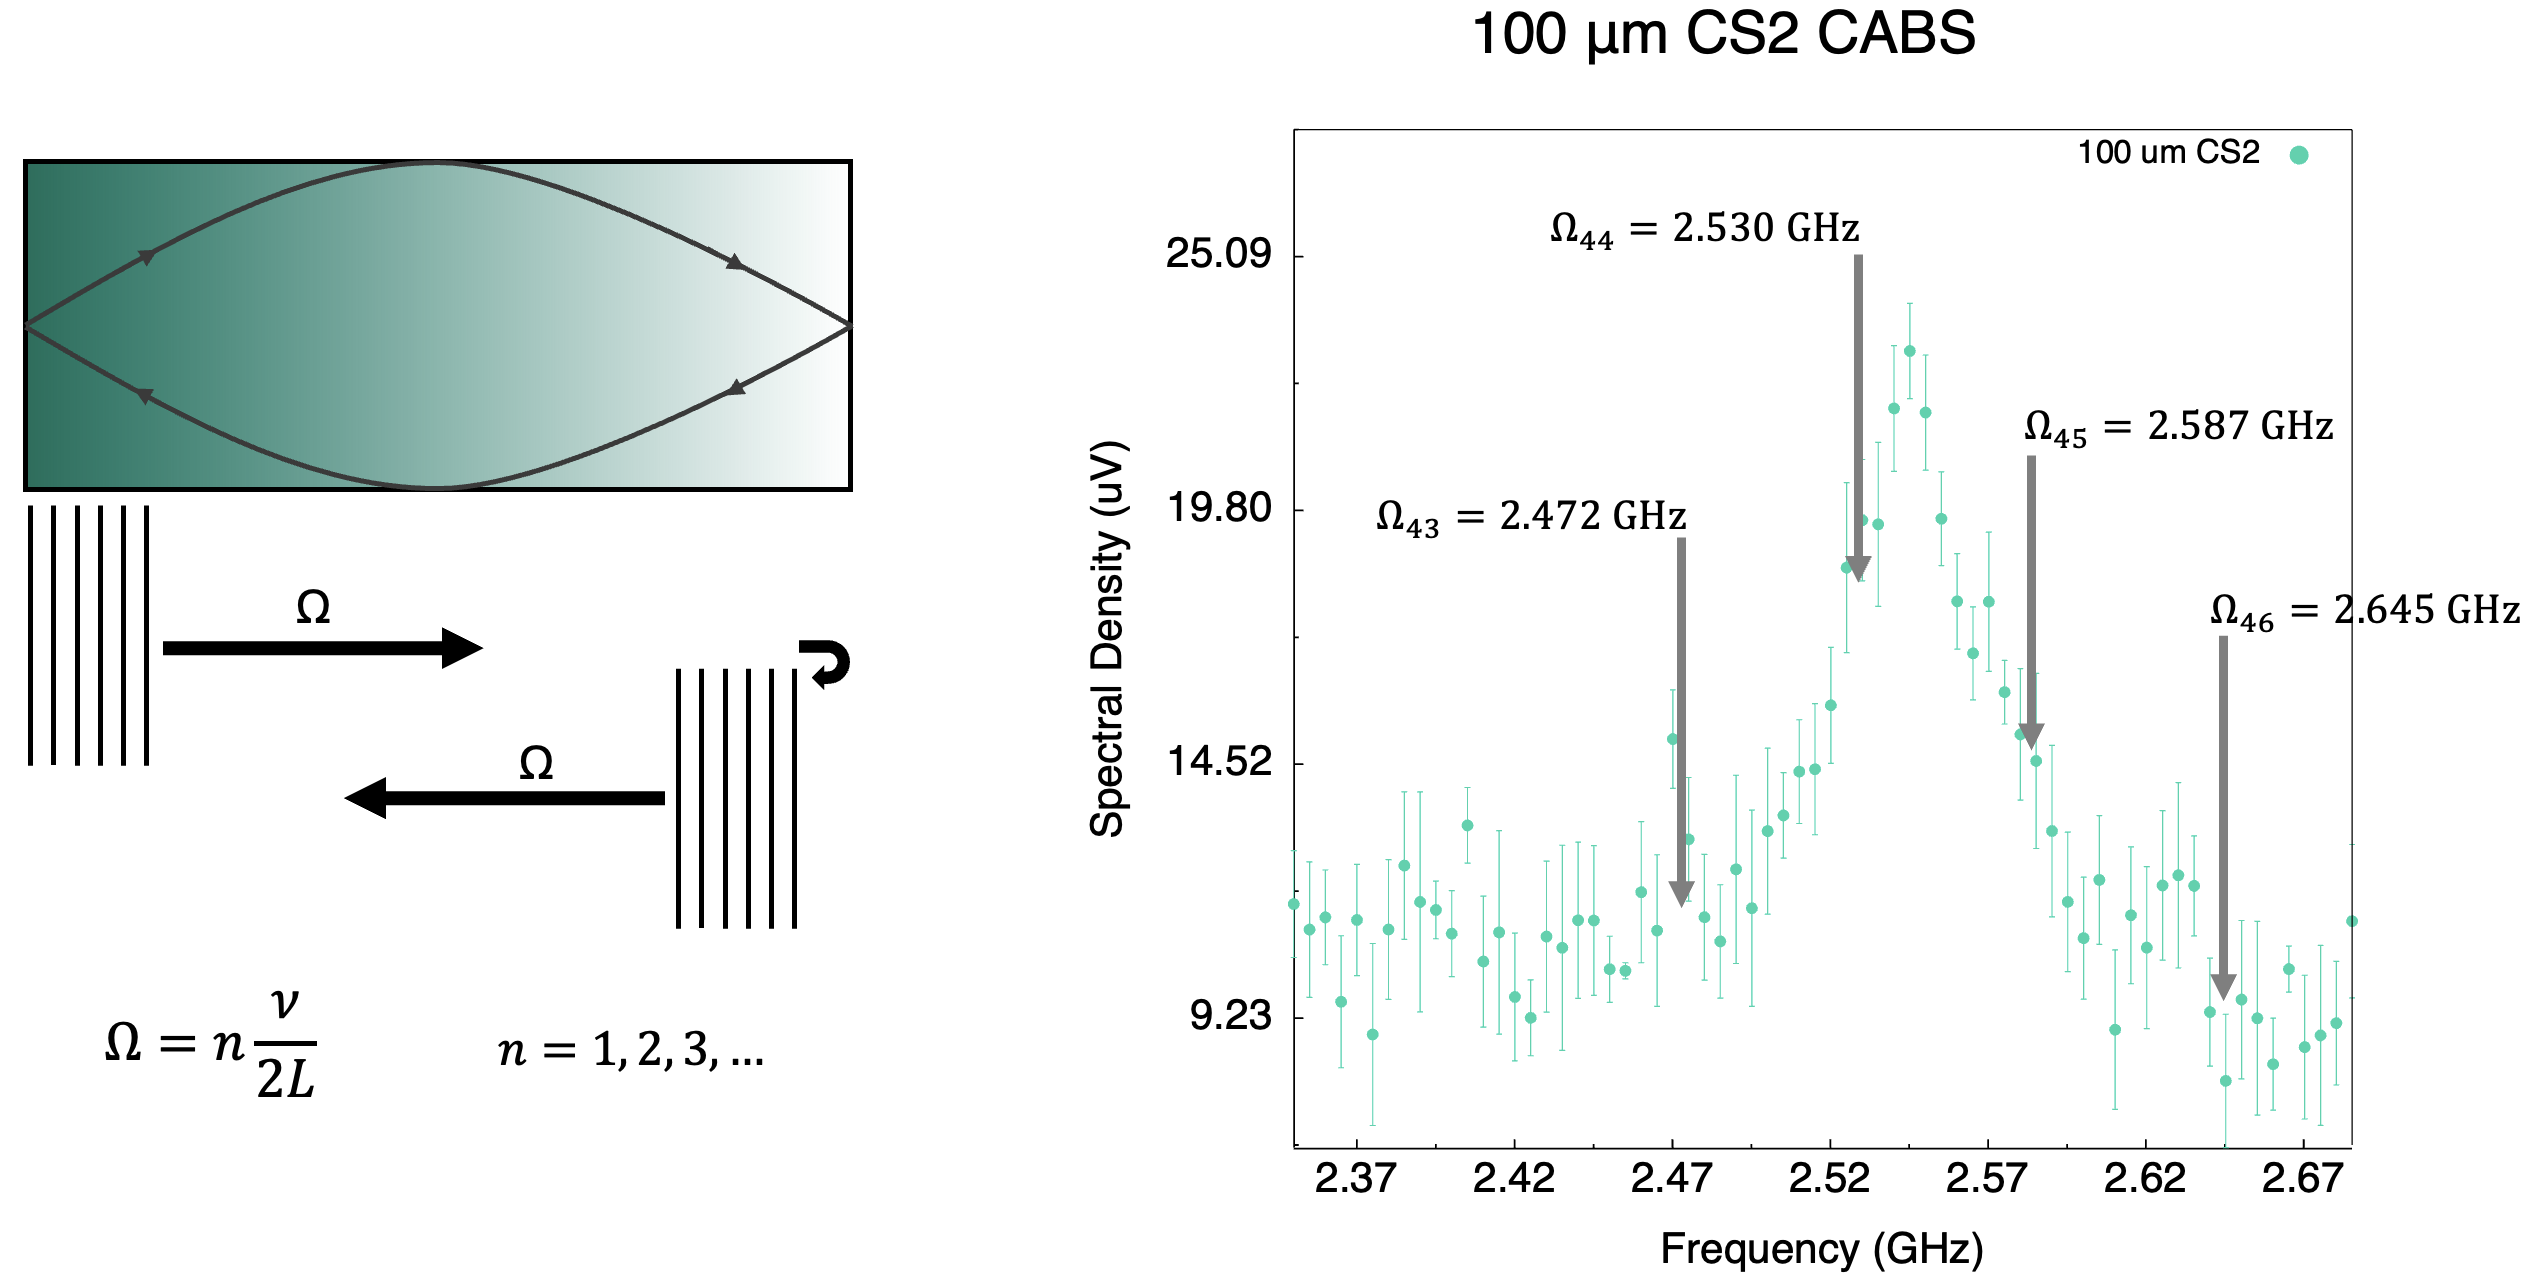
\includegraphics[width=\textwidth]{figs/4-Raman/HowWouldRamanModesAppear.png}
  \caption{How would Raman modes appear.}
  \label{fig:HowWouldRamanModesAppear}
\end{figure}

%--------------------------------------------------------------------%

\section{Discussion}
\label{sec:Raman:Discussion}

\subsection{Pathways to Brillouin-Induced Raman Modes}
\label{subsec:Raman:Pathways}
Ideal platforms by category
  waveguide - long TeO2 rib, evenly spaced square holes
  TeO2 thin film/crystal - dissolve only small area of substrate for beam spot
  CS2 cell - 5um
  Fiber - notched, acoustic fiber Bragg grating

\subsection{Conclusion}
\label{subsec:Raman:Conclusion}

\begin{itemize}
\item \textbf{Connection to Dissertation Theme}
  \begin{itemize}
    \item Relate back to the broader aims of controlling phonons at room temperature, highlighting how these efforts extend your dissertation’s exploration of optomechanical interactions.
  \end{itemize}
\end{itemize}

\clearpage
\thispagestyle{empty}
\null
\newpage
